\documentclass[11pt]{article}

% AMS Packages
\usepackage{amsmath} 
\usepackage{amssymb} 
\usepackage{amsthm}
% Page dimensions
\usepackage[margin=1in]{geometry}
% Images
\usepackage[pdftex]{graphicx} 
% Enumerate package
\usepackage{enumitem} 
\usepackage{array} 
% Fancify pages
\usepackage{fancyhdr} 
% Convert captions on figures to bold font
\usepackage[labelfont=bf,textfont=md]{caption}
% Time New Roman font
\usepackage{times}

\usepackage{setspace} 
% SI Units in math type
\usepackage{siunitx}
\usepackage{textcomp} 
% Change sizes of sections
\usepackage{titlesec}
\titleformat{\section}{\normalfont\large\bfseries}{\thesection}{1em}{}
\titleformat{\subsection}{\normalfont\bfseries}{\thesubsection}{1em}{}
\titleformat{\subsubsection}{\normalfont\small\bfseries}{\thesubsubsection}{1em}{}
% Declare useful math operators
\DeclareMathOperator*{\argmin}{arg\,min}
\DeclareMathOperator*{\plim}{plim}
\DeclareMathOperator{\Tr}{Tr}

\usepackage{tikz}
\usetikzlibrary{shapes.geometric, arrows}

% title
\title{Synaptic weight diversity enhances encoding and decoding in a linear-nonlinear network}
\date{}
\begin{document}
	\maketitle
	
	\section{Introduction}
	\begin{figure}[ht]
	\centering
	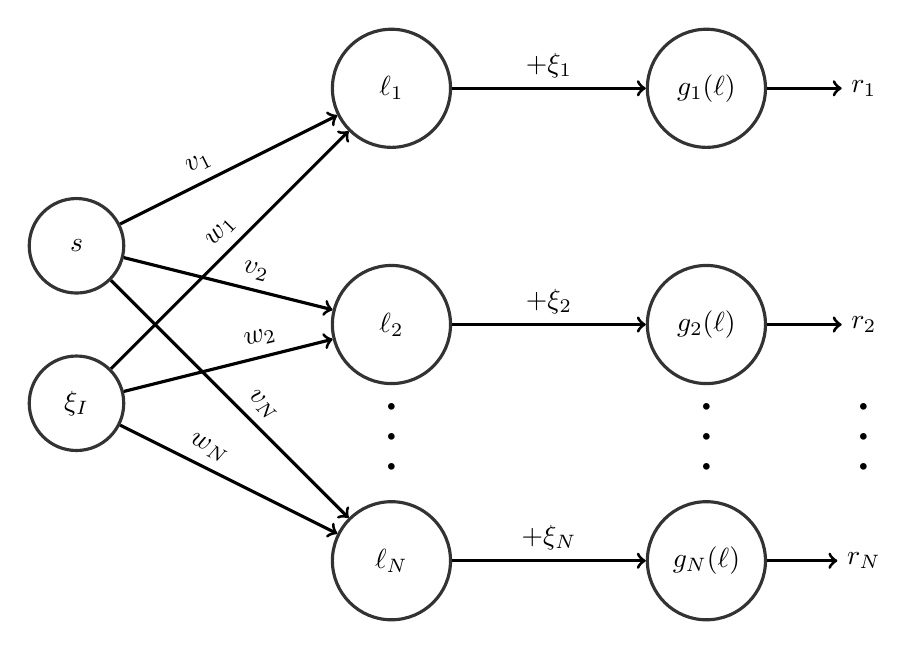
\begin{tikzpicture}
	\tikzstyle{main} = [circle, minimum size = 12mm, line width = 0.4mm, draw=black!80, node distance = 16mm]
	\tikzstyle{main2} = [circle, minimum size = 15mm, line width = 0.4mm, draw=black!80, node distance = 16mm]
	\node[main, fill = white!100] at (0, 1.) (s) {$s$};
	\node[main, fill = white!100] at (0, -1.) (inj) {$\xi_I$};
	\node[main2] at (4.,3.0)  (lin1) {$\ell_1$};
	\node[main2] at (4.,0.0)  (lin2) {$\ell_2$};
	\node[main2] at (4,-3.0) (linN) {$\ell_{N}$};
	
	\node[main2] at (8, 3.0) (nonlin1) {$g_1(\ell)$};
	\node[main2] at (8, 0.0) (nonlin2) {$g_2(\ell)$};
	\node[main2] at (8, -3.0) (nonlinN) {$g_N(\ell)$};
	
	\node at (10, 3.0) (r1) {$r_1$};
	\node at (10, 0.0) (r2) {$r_2$};
	\node at (10, -3.0) (rN) {$r_N$};
	
	\draw[->, line width = 0.4mm] (s) -- (lin1) node[midway, above left, sloped] {$v_1$};
	\draw[->, line width = 0.4mm] (s) -- (lin2) node[midway, above right, sloped] {$v_2$};
	\draw[->, line width = 0.4mm] (s) -- (linN) node[midway, above right, sloped] {$v_N$};
	
	\draw[->, line width = 0.4mm] (inj) -- (lin1) node[pos = 0.6, above left, sloped] {$w_1$};
	\draw[->, line width = 0.4mm] (inj) -- (lin2) node[pos = 0.8, above left, sloped] {$w_2$};
	\draw[->, line width = 0.4mm] (inj) -- (linN) node[midway, above left, sloped] {$w_N$};
	
	\draw[->, line width = 0.4mm] (lin1) -- (nonlin1) node[midway, above] {$+\xi_1$};
	\draw[->, line width = 0.4mm] (lin2) -- (nonlin2) node[midway, above] {$+\xi_2$};
	\draw[->, line width = 0.4mm] (linN) -- (nonlinN) node[midway, above] {$+\xi_N$};
	
	\draw[->, line width = 0.4mm] (nonlin1) -- (r1);
	\draw[->, line width = 0.4mm] (nonlin2) -- (r2);
	\draw[->, line width = 0.4mm] (nonlinN) -- (rN);
	
	\path (lin2) -- (linN) node [black, font=\Huge, midway, sloped] {$\dots$};
	\path (nonlin2) -- (nonlinN) node [black, font=\Huge, midway, sloped] {$\dots$};
	\path (r2) -- (rN) node [black, font=\Huge, midway, sloped] {$\dots$};	
	\end{tikzpicture}
	\caption{Linear-Nonlinear Network Architecture}
	\end{figure}
	\section{Fisher Information, First Stage}
	We can calculate the Fisher information after the first stage. 
	
	\section{Mutual Information}
	
	
	\appendix
	\newpage
	\section{Calculation of Conditional and Marginal Probability Distributions}
	We present the calculation of the conditional and marginal probability distributions after the linear stage of computation. Recall that the output of the $i$th neuron in the linear stage can be written as
	\begin{align}
		\ell_i &= v_i s + w_i \sigma_I \xi_I + \sigma_G\xi_i
	\end{align}
	and thus the overall population can be written as 
	\begin{align}
		\boldsymbol{\ell} &= \mathbf{v} s + \mathbf{w} \sigma_I \xi_I + \sigma_G \boldsymbol{\xi}.
	\end{align}
	
	\subsection{Conditional Distribution $P[\boldsymbol{\ell}|s]$}
	Conditioning on the stimulus and injected noise value establishes independence between the neural activity $\ell_i$. Thus, we obtain $P[\boldsymbol{\ell}|s]$ by marginalizing the distribution $P[\boldsymbol{\ell}|s,\xi_I]$ over the injected noise $\xi_I$:
	\begin{align}
	P[\boldsymbol{\ell}|s] &= \int P[\boldsymbol{\ell}|s, \xi_I] P[\xi_I]d\xi_I \\
	&= \int d\xi_I  \frac{1}{\sqrt{2\pi}} \exp(-\xi_I^2/2) \prod_{i=1}^N P[\ell_i|s,\xi_I] \\
	&=  \frac{1}{\sqrt{2\pi}} \int d\xi_I   \exp(-\xi_I^2/2) \prod_{i=1}^N \frac{1}{\sqrt{2\pi \sigma_G^2}} \exp\left(-\frac{\left(\ell_i - (v_i s + \sigma_I w_i \xi_I)\right)^2}{2\sigma_G^2}\right) \\
	&= \frac{1}{(2\pi)^{(N+1)/2}\sigma_G^N} \int d\xi_I \exp(-\xi_I^2/2) \exp\left(-\frac{1}{2\sigma_G^2}\sum_{i=1}^N \left(\ell_i - (v_i s + \sigma_I w_i \xi_I)\right)^2\right) \\
	&= \frac{1}{(2\pi)^{(N+1)/2}\sigma_G^N} \int d\xi_I \exp(-\xi_I^2/2) \notag \\
	& \qquad \times \exp\left(-\frac{1}{2\sigma_G^2}\sum_{i=1}^N \ell_i^2 -2\ell_i (v_i s + \sigma_I w_i \xi_I) + (v_i s + \sigma_I w_i \xi_I)^2\right) \\
	&= \frac{1}{(2\pi)^{(N+1)/2}\sigma_G^N} \exp\left(-\frac{1}{2\sigma_G^2}\sum_{i=1}^N \ell_i^2\right)\exp\left(\frac{s}{\sigma_G^2}\sum_{i=1}^N \ell_i v_i \right)\exp\left(-\frac{1}{2\sigma_G^2}s^2 \left\{v\right\}_2\right) \notag \\
	&\times \int d\xi_I\exp\left[-\frac{1}{2}\left(1+\frac{\sigma_I^2}{\sigma_G^2} \left\{w\right\}_2\right)\xi_I^2 +\frac{\sigma_I}{\sigma_G^2}\left( \sum_{i=1}^N \ell_i w_i - s \left\{v,w\right\}_{1,1}\right)\xi_I \right] \\
	&=  \frac{1}{(2\pi)^{(N+1)/2}\sigma_G^N}\exp\left(-\frac{1}{2\sigma_G^2}\sum_{i=1}^N \ell_i^2\right)\exp\left(\frac{s}{\sigma_G^2}\sum_{i=1}^N \ell_i v_i \right)\exp\left(-\frac{1}{2\sigma_G^2}s^2 \left\{v\right\}_2\right) \notag \\
	&\qquad \times \frac{\sqrt{2\pi \sigma_G^2}}{\sqrt{\sigma_G^2 + \sigma_I^2 \left\{w\right\}_2}}\exp\left[\frac{\sigma_I^2\left(\displaystyle\sum_{i=1}^N \ell_i w_i - s  \left\{v,w\right\}_{1,1}\right)^2}{2 \sigma_G^2 (\sigma_G^2 + \sigma_I^2 \left\{w\right\}_2)}\right],
	\end{align}
	which we can write concisely as
	\begin{align}
		P[\boldsymbol{\ell}|s] &= \frac{1}{\sigma_G^{N-1} \sqrt{(2\pi)^N(\sigma_G^2 + \sigma_I^2 ||\mathbf{w}||^2)}} \exp\left[-\frac{1}{2\sigma_G^2} (\boldsymbol{\ell} - \mathbf{v}s)^T\left(\mathbf{I} - \frac{\sigma_I^2 \mathbf{ww}^T}{\sigma_G^2 + \sigma_I^2 ||\mathbf{w}||^2}\right) (\boldsymbol{\ell} - \mathbf{v}s) \right] \notag 
	\end{align}
	
	\section{Calculation of Mutual Information}
	In this section we calculate the mutual information $I[s,\boldsymbol{\ell}]$ between the stimulus $s$ and the output of the linear layer $\boldsymbol{\ell}$. 
	
	Recall that the output of the $i$th neuron can be written as 
	\begin{align}
	r_i &= g_i(\ell_i) \\
	&= g_i(v_i s + \sigma_I w_i \xi_I + \sigma_G\xi_i).
	\end{align}
	Ultimately, we want $I[s, \mathbf{r}]$. For now, we will focus on $I[s, \boldsymbol{\ell}]$ and note that $I[s,\mathbf{r}] \leq I[s, \boldsymbol{\ell}]$ by the data processing inequality. To calculate the mutual information, we must first calculate $P[\boldsymbol{\ell}|s]$. We can do this via marginalization:
\end{document}
